\documentclass[11pt]{standalone}
\usepackage[T1]{fontenc}
\usepackage{pgfplots}

\pgfplotsset{
  compat=newest,
  xlabel near ticks,
  ylabel near ticks
}

\begin{document}
  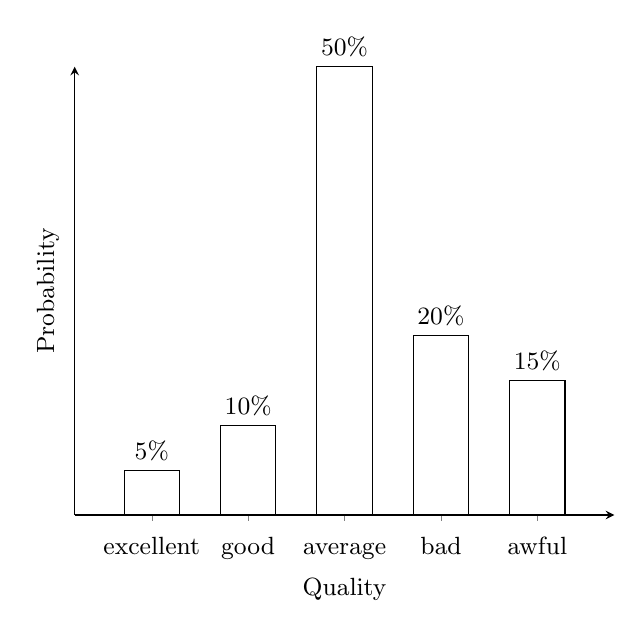
\begin{tikzpicture}[font=\small]
    \begin{axis}[
      ybar,
      bar width=20pt,
      xlabel={Quality},
      ylabel={Probability},
      ymin=0,
      ytick=\empty,
      xtick=data,
      axis x line=bottom,
      axis y line=left,
      enlarge x limits=0.2,
      symbolic x coords={excellent,good,average,bad,awful},
      xticklabel style={anchor=base,yshift=-\baselineskip},
      nodes near coords={\pgfmathprintnumber\pgfplotspointmeta\%}
    ]
      \addplot[fill=white] coordinates {
        (excellent,5)
        (good,10)
        (average,50)
        (bad,20)
        (awful,15)
      };
    \end{axis}
  \end{tikzpicture}
\end{document}

